% STEP 1: Choose oneside or twoside. Use the 'draft' option a lot when writing.
\documentclass[english, oneside]{HYgradu}

\usepackage[utf8]{inputenc} % For UTF8 support. Use UTF8 when saving your file.
\usepackage{lmodern} % Font package
\usepackage{textcomp}
\usepackage[pdftex]{color, graphicx} % For pdf output and jpg/png graphics
\usepackage[pdftex, plainpages=false]{hyperref} % For hyperlinks and pdf metadata
\usepackage{fancyhdr} % For nicer page headers
%\usepackage{tikz} % For making vector graphics (hard to learn but powerful)
%\usepackage{wrapfig} % For nice text-wrapping figures (use at own discretion)
\usepackage{amsmath, amssymb} % For better math
\usepackage[sort,colon]{natbib} % For bibliography
\usepackage[bf]{caption} % For more control over figure captions
\usepackage{marginnote} % margin notes for myself
%\usepackage{svg} % vector graphics
\usepackage{graphicx}
\graphicspath{{kuvat/tex/}}

% titlesec and fix for no numbering on titlesec 2.10.2
\usepackage{titlesec}
\usepackage{etoolbox}
\makeatletter
\patchcmd{\ttlh@hang}{\parindent\z@}{\parindent\z@\leavevmode}{}{}
\patchcmd{\ttlh@hang}{\noindent}{}{}{}
\makeatother

\fussy % Probably not needed but you never know...

\renewcommand{\topfraction}{.75} % less single-float pages
\renewcommand{\floatpagefraction}{.75} % less single-float pages


% näillä subsubsubsection käyttöön
%\titleclass{\subsubsubsection}{straight}[\subsection]
%\newcounter{subsubsubsection}[subsubsection]
%\renewcommand\thesubsubsubsection{\thesubsection.\arabic{subsubsubsection}}
%\titleformat{\subsubsubsection}
%  {\normalfont\normalsize\bfseries}{\thesubsubsubsection}{1em}{}
%\titlespacing*{\subsubsubsection}
%{0pt}{3.25ex plus 1ex minus .2ex}{1.5ex plus .2ex}
%\makeatletter
%\def\toclevel@subsubsubsection{3}
%\def\l@subsubsubsection{\@dottedtocline{4}{7em}{4em}}
%\@addtoreset{subsubsubsection}{section}
%\@addtoreset{subsubsubsection}{subsection}
%\makeatother
%\setcounter{secnumdepth}{3}
%\setcounter{tocdepth}{4}

% OPTIONAL STEP: Set up properties and metadata for the pdf file that pdfLaTeX makes.
% But you don't really need to do this unless you want to.
%\hypersetup{
%    bookmarks=true,         % show bookmarks bar first?
%    unicode=true,           % to show non-Latin characters in Acrobat’s bookmarks
%    pdftoolbar=true,        % show Acrobat’s toolbar?
%    pdfmenubar=true,        % show Acrobat’s menu?
%    pdffitwindow=false,     % window fit to page when opened
%    pdfstartview={FitH},    % fits the width of the page to the window
%    pdftitle={},            % title
%    pdfauthor={},           % author
%    pdfsubject={},          % subject of the document
%    pdfcreator={},          % creator of the document
%    pdfproducer={pdfLaTeX}, % producer of the document
%    pdfkeywords={something} {something else}, % list of keywords for
%    pdfnewwindow=true,      % links in new window
%    colorlinks=true,        % false: boxed links; true: colored links
%    linkcolor=black,        % color of internal links
%    citecolor=black,        % color of links to bibliography
%    filecolor=magenta,      % color of file links
%    urlcolor=cyan           % color of external links
%}

% STEP 2:
% Set up all the information for the title page and the abstract form.
% Replace parameters with your information.
\title{Your Title Here}
\author{Anni Järvenpää}
\date{\today}
\level{Master's thesis}
\faculty{Faculty of Science}
\department{Department of Physics}
\address{PL 64 (Gustaf Hällströmin katu 2a)\\00014 University of Helsinki}
\subject{Astronomy}
\prof{Associate Professor Peter Johansson}{Dr. Till Sawala}
\censors{prof. Smith}{doc. Smythe}{}
\depositeplace{}
\additionalinformation{}
\numberofpagesinformation{\numberofpages\ pages}
\classification{}
\keywords{Your keywords here}
\quoting{}%``Bachelor's degrees make pretty good placemats if you get them laminated.'' \\---Jeph Jacques}
% There is a way out of every box, a solution to every puzzle; it's just a matter of finding it
% Things are only impossible until they're not

\begin{document}

% Generate title page.
\maketitle

% STEP 3:
% Write your abstract (of course you really do this last).
% You can make several abstract pages (if you want it in different languages),
% but you should also then redefine some of the above parameters in the proper
% language as well, in between the abstract definitions.
\begin{abstract}
Abstract goes here.
\end{abstract}

% Place ToC
\mytableofcontents



% -----------------------------------------------------------------------------------
% STEP 4: Write the thesis.
% Your actual text starts here. You shouldn't mess with the code above the line except
% to change the parameters. Removing the abstract and ToC commands will mess up stuff.
\chapter{Introduction}

\section{TL;DR version of prerequisite information}
\begin{enumerate}
	\item galaxies form
	\begin{itemize}
		\item Why?
		\item When?
		\item How?
		\item Where?
	\end{itemize}
	\item galaxies form in groups
	\item our local group is one of these
	\item something about large scale distribution of galaxies
\end{enumerate}

\section{History of Local Group Research}
LG objects visible with naked eye -> realization they are something outside our galaxy -> realization they are something very much like our galaxy

First determining distance was difficult, now mass is more interesting question

\section{Aim of This Thesis}
Whatever the main results end up being, presented in somewhat coherent manner and hopefully sugar-coated enough to sound Important and Exciting.


\chapter{Theoretical Background}
Think whether LG or LCDM first
%theorythingies from Fattahi paper introduction
\section{Local Group}
Definition of galaxy group, our local group is one of these.

Mass estimate (Li, Yang masses for the LG and MW)

Maybe something about scale of things in our universe, what are galaxy groups made of, what do you get if you go one distance scale up, what's different in galaxy clusters

\subsection{Structure}
Galaxies that are part of LG, distribution of smaller ones around bigger ones

Current mass estimates (at least timing argument, hubble flow and maybe satellites)

\subsection{Evolution}
How have we ended up in a situation described earlier? What will happen in future?


\section{Expanding universe}
\subsection{Discovery}
Make maths, add cosmological constant, make observations, remove cosmological constant

Enough cosmology here or in other sections to make other parts of thesis to make sense and to suffice as master's thesis = basic textbook cosmology and galaxy formation theory %t. puppe
\subsection{$\Lambda$CDM Cosmology}


\subsection{Hubble flow}
What is, where seen, what means, how to measure, hotness/coldness

Plot: observations with fitted hubble flow


\chapter{general simulation thingies}
Data used here from EAGLE which uses modified GADGET-2 which is a tree-code that uses leapfrog
\section{N-body simulations}
\subsection{Hierarchical Tree Algorithm}
\subsection{Numerical Integrators}
\subsection{Halo Finding with Subfind} %iannuzzi thesis
%merger tree mentioned in todo, is it relevant?

\section{Description of actual simulations used}
Volume, number of particles, compare to other simulations, where better and where maybe worse

Resimulation of interesting regions

Simulation has same parameters as EAGLE
800 Mpc volume used
schaye 2015 paper
DM-only parts: Volker-Springer Gadget and Gadget 2 papers 1999 and 2005 or something,     gravity part is more interesting than SPH 
Zooms can use multiple meshes, only one is used here
gravitational softening


\chapter{Mathematical and statistical methods}
\reversemarginpar
\marginnote{\footnotesize{TODO: merkkaa heti alkuun kenen lähestymistapaa aiot seurailla}}
täällä tarvittavat esitiedot ja önnönnöö, listaa mm. mitä aiot kertoa kunhan tiedät itsekään

\section{Statistical Background}
\reversemarginpar
\marginnote{\footnotesize{vähän parempi tässä kuin aiemman otsikon alla}}
Precision of the used equipment limits accuracy of all data gathered from physical experiments, simulations or observations. Therefore the results are affected by the measurement process and the results have to be presented as estimates with some error, magnitude of which is affected by both number of data points and accuracy of the measurement equipment. \citep{bohm2010introduction}

Estimating errors for measured quantities offers a way to test hypotheses and compare different experiments. This is done using different statistical methods, of which the most relevant for this thesis are covered here. The methods used in this work are shortly introduced in the following sections together with basic statistical concepts that are necessary to understand the methods. \citep{bohm2010introduction}



\subsection{Hypothesis testing and p-values}
A common situation in scientific research is that one has to compare a sample of data points to either a model or another sample in order to derive a conclusion from the dataset. In statistics, this is known as hypothesis testing. For example, this can mean testing hypotheses such as ''these two variables are not correlated'' or ''this sample is from a population with a mean of 1.0''. \citep{wall2003practical} Next paragraphs shortly introduce the basic concept of hypothesis testing and methods that can used to test the hypothesis ''these two samples are drawn from the same distribution''.

Typically the process of hypothesis testing begins with forming of a null hypothesis $H_0$ that is formatted such that the aim for the next steps is to either reject it or deduce that it cannot be rejected with a chosen significance level. Negation of the null hypothesis is often called research hypothesis or alternative hypothesis and denoted as $H_1$. For example, this can lead to $H_0$ ''this dataset is sampled from a normal distribution'' and $H_1$ ''this dataset is not sampled from a normal distribution''. Choosing the hypothesis in this manner is done because often the research hypothesis is difficult to define otherwise. \citep{bohm2010introduction, wall2003practical}

After setting the hypothesis one must choose an appropriate test statistic. Ideally this is chosen such that the difference between cases $H_0$ and $H_1$ is as large as possible. Then one must choose 
the significance level $\alpha$ which corresponds to the probability of rejecting $H_0$ in the case where $H_0$ actually is true. This fixes the critical region i.e. the values of test statistic that lead to the rejection of the $H_0$. \citep{bohm2010introduction, wall2003practical}

\reversemarginpar
\marginnote{\footnotesize{miten $\alpha$ valitaan, millaiset arvot ovat tyypillisiä? miten $\alpha$ -> critical value -> rejection/no rejection. otoskoko = N mukaan tänne}}
It is crucial not to look at the test results before choosing $\alpha$ in order to avoid intentional or unintentional fiddling with the data or changing the criterion of acceptance or rejectance to give desired results. Only after these steps should the test statistic be calculated. If the test statistic falls within the critical region, $H_0$ should be rejected and otherwise stated that $H_0$ cannot be rejected at this significance level. \citep{bohm2010introduction, wall2003practical}

This kind of probability based decision making is always prone to error. It is easy to see that $\alpha$ corresponds to the chance of $H_0$ being rejected when it is true. This is known as error of the first kind. However, this is not the only kind of error possible. It might also occur that $H_0$ is false but it does not get rejected, which is known as error of the second kind. \citep{bohm2010introduction}

Despite statistical tests having a binary outcome ''$H_0$ rejected'' or ''$H_0$ not rejected'', a continuous output is often desired. This is what p-values are used for. The name p-value hints towards probability, but despite it's name p-value is not equal to the probability that the null hypothesis is true. These p-values are functions of a test statistic and the p-value for a certain value $t_{obs}$ of a test statistic gives the probability that under the condition that $H_0$ is true, the value of a test statistics for a randomly drawn sample is at least as extreme as $t_{obs}$. Therefore if p-value is smaller than $\alpha$, $H_0$ is to be rejected. \citep{bohm2010introduction}

\subsection{Distribution functions}
\reversemarginpar
\marginnote{\footnotesize{ei hyvä, harkitse esim http://puppu\-lause\-generaattori.fi/?ava\-in\-sana=ja\-kau\-ma\-funk\-tio}}
Some statistical tests such as the Kolmogorov-Smirnov test and the Anderson-Darling test make use of distribution functions such as cumulative density function (CDF) and empirical distribution function (EDF) in determining the distribution from which a sample is drawn. %Therefore it is important to grasp these concepts in order to fully understand these tests. [this is shit t. puppe]

To understand CDF and EDF, one must first be familiar with probability density function (PDF).
\reversemarginpar
\marginnote{\footnotesize{PDF määritelmä vaikea ymmärtää}}[0.5cm]
As the name suggests, PDF is a function the value of which at some point $x$ represents the likelihood that the value of the random variable would equal $x$. This is often denoted $f(x)$. Naturally for continuous functions the probability of drawing any single value from the distribution is zero, so these values should be interpreted as depicting relative likelihoods of different values. For example if $f(a)=0.3$ and $f(b)=0.6$ we can say that drawing value $b$ is twice as likely as drawing value $a$. \citep{htk}

Another way to use the PDF is to integrate it over semi-closed interval from negative infinity to some value $a$ to obtain the CDF, often denoted with $F(x)$:
\begin{equation}
	F(x) = \int_{-\infty}^x f(x') \,dx'.
\end{equation}	
This gives the probability of a random value drawn from the distribution having value that is smaller than $x$. Relation between the PDF and the CDF is illustrated in figure \ref{fig:cdf}, where PDFs and CDFs are shown for three different distributions. It is easy to see the integral relation between PDF and CDF and how wider distributions have wider CDFs. \citep{htk}

\begin{figure}
   \reversemarginpar
	\marginnote{\footnotesize{lisää johonkin selitys normaalijakauman parametreille}}
   \centering
   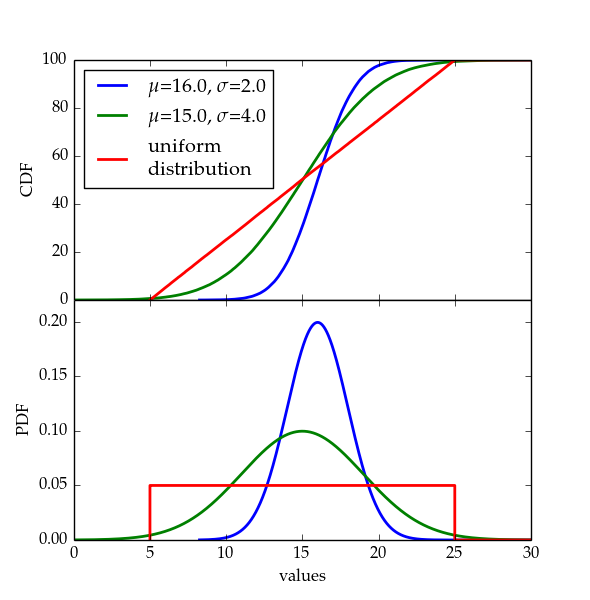
\includegraphics[width=0.9\textwidth]{kuvat/cdf.png}
   \caption{Cumulative distribution function (top panel) for three random samples (PDFs shown in the bottom panel) drawn from different distributions, two of which are normal and one is uniform.}
   \label{fig:cdf}

\end{figure}

\reversemarginpar
\marginnote{\footnotesize{esittelet nyt nolosti EDF:n nimeltä kahdesti, mieti ratkaisu}}
Both the PDF and the CDF apply to whole population or the set of all possible outcomes of a measurement. In reality the sample is almost always smaller than this. Therefore one cannot measure the actual CDF. Nevertheless, it is possible to calculate a similar measure of how big a fraction of measurements falls under a given value. This empirical counterpart of the CDF is known as empirical distribution function (EDF), often denoted $\hat F(x)$, and for a dataset $X_1, X_2,\,..., X_n$ containing $n$ samples it is defined to be
\begin{equation}
	\hat F(x) = \frac{1}{n}\sum_{i=1}^n I[X_i \leq x]
\end{equation}
where $I$ is the indicator function, value of which is 1 if the condition in brackets is true, otherwise 0. \citep{feigelson2012modern}

Due to the EDF being a result of random sampling, it may deviate from the underlying CDF considerably as can be seen by comparing CDFs in figure \ref{fig:cdf} and corresponding EDFs in figure \ref{fig:edf}. The latter figure also has EDFs corresponding to two random samples drawn from the distribution of the green curve in the first figure to further illustrate the differences that can arise from random sampling. This randomness also makes determining whether two samples are drawn from the same distribution difficult.

\reversemarginpar
\marginnote{\footnotesize{kerro, miten sample size suhteutuu oikeaan käsiteltyyn dataan}}
\begin{figure}
   \centering
   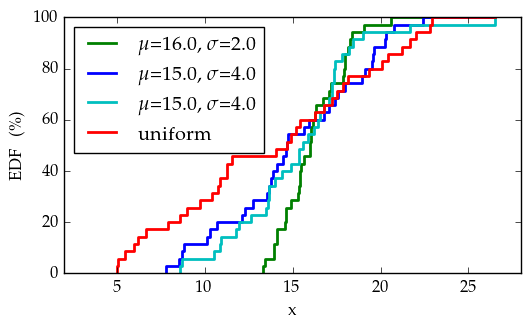
\includegraphics[width=0.9\textwidth]{kuvat/edf.png}
   \caption{Empirical distribution function for four random samples (N=35) drawn from the same distributions as in figure \ref{fig:cdf}. Note that both the blue and the cyan data are drawn from the same distribution.}
   \label{fig:edf}
\end{figure}


\section{Regression Analysis}
line fitting and other trivial things

Ordinary least squares: mitä, miksi ongelmallinen -> total (orthogonal?) least squares (= ensimmäinen principal component kahdessa ulottuvuudessa) 

%\subsection{Ordinary Least Squares}

%\subsection{


\section{Principal Component Analysis}
Principal component analysis (PCA) is a statistical procedure first introdueced by \citet{pearson1901lines} to aid physical, statistical and biological investigations where fitting a line or a plane to n-dimensional dataset is desired. This approach also solves the problem of sometimes arbitrary choice of dividing the data to dependent and independent variables introduced in section 4.2.something. %TODO

\reversemarginpar
\marginnote{\footnotesize{not sure if kannattaa kuvaille proseduuria erityisen tarkkaan, selityksestä tulee pitkällinen jos aikoo aloittaa keskimääräisen tähtitieteilijän lähtötasolta, ehkä vain ohjaa lähteeseen}}
PCA can be used to both reduce and interpret data \citep{johnson1988applied}. Often PCA alone does not produce the desired result, but instead its output is used as a starting point for other analysis methods such as factor analysis or multiple regression. These applications are introduced in the following subsections together with a short description of performing PCA and interpreting its results.

\subsection{Extracting Principal Components}

\subsection{Applications in Factor Analysis}

\subsection{Principal Component Regression}

\section{Error analysis}

%\section{Goodness of fit testing}
%nyt tarvitsen uuden aloituskappaleen


\section{Comparing two samples drawn from unknown distributions}
\reversemarginpar
\marginnote{\footnotesize{TODO: oispa parempi otsikko. mieti, onko tämä muutenkaan hyvä nyt kun on siirretty yksi otsikkotaso ylöspäin}}[-3cm]
\marginnote{\footnotesize{selitä categorical data}}[2.2cm]
A common question in multiple fields of science is whether two or more samples are drawn from the same distribution. This can occur for example when comparing effectiveness of two procedures, determining if the instrument has changed over time or whether observed data is compatible with simulations. There are multiple two-sample tests that can address this kind of questions, e.g. $\chi^2$, Kolmogorov-Smirnov, Cram\'er-von Mises and Anderson-Darling tests. \citep{bohm2010introduction, feigelson2012modern}

In addition to comparing two samples, these tests can be used as one-sample tests to determine whether it is expected that the sample is from a particular distribution. However, some restrictions apply when using the one-sample variants. Some of these tests use categorical data, for example ''number of galaxies that are active'' or ''number of data points between values 1.5 and 1.6'' and compares numbers of samples in different categories, whereas the others are applied to numerical data and compare empirical distribution functions (EDF) of the datasets. \citep{feigelson2012modern}


\subsection{$\chi^2$ test}
\reversemarginpar
\marginnote{\footnotesize{keksi paremmat esimerkit koko kappaleeseen, jotain relevanttia myöhempää tutkimusta ajatellen. katso kommentit paperista sen jälkeen, kaikkia ei täällä vielä}}
Astronomical data often involves classifying objects into categories such as ''stars with exoplanets'' and ''stars without exoplanets'' or the spectral classes of stars. One tool for analyzing such categorical data is $\chi^2$ test. It can be used both to determine whether a sample can be drawn from a certain distribution and to test whether two samples can originate from a single distribution. \citep{feigelson2012modern, corder2014nonparametric}

For one-sample test, the $\chi^2$ test uses the number of measurements in each bin together with a theoretical estimate calculated from the null hypothesis. For example one might have observed exoplanets and tabulated the number of planet-hosting stars of different spectral class as is shown in table \ref{tab:exoplanets} and now wants 
to test the observations against null hypothesis ''Distribution of stellar classes for observed exoplanet-hosting stars is equal to that of main sequence stars in solar neighbourhood as given by \citet{ledrew2001real}'' using significance level $\alpha=0.01$. The data is categorical, so now $\chi^2$ test is a justified choice. \citep{corder2014nonparametric}

\begin{table}
	\centering
	\begin{tabular}{p{2cm}|p{4cm}}
		Stellar class & Number of observed planetary systems \\ \hline
		A & 6 \\
		F & 38 \\
		G & 39 \\
		K & 134
	\end{tabular}
	\caption{Example of categorical data.}
	\label{tab:exoplanets}
\end{table}

\begin{table}
	\centering
	\begin{tabular}{ l | l | l }
		Stellar class & Observations ($f_o$)& Theory ($f_e$) \\ \hline
		A & 6 & 6 \\
		F & 38 & 28 \\
		G & 39 & 71 \\
		K & 134 & 112 \\ \hline
		total & 217 & 217
	\end{tabular}
	\caption{Data of table \ref{tab:exoplanets} together with expected values if null hypothesis was true.}
	\label{tab:exoplanets-null}
\end{table}

In this case the first step would be to calculate the expected observation counts for each bin according to the null hypothesis. Table \ref{tab:exoplanets-null} contains these expected counts ($f_e$) together with the observations ($f_o$). These observed and expected values are then used to calculate the $\chi^2$ test statistic, defined as
\begin{equation}
	\chi^2 = \sum_i \frac{(f_o - f_e)^2}{f_e}.
\end{equation}
\reversemarginpar
\marginnote{\footnotesize{mistä kriittisiä arvoja voi lukea ja mistä sain omani, onhan selitetty (tässä tai) aiemmin}}
In this case, one gets $\chi^2 \approx 23.6$. The data has four bins, so the degree of freedom is $4-1=3$. Next one can compare the calculated $\chi^2$ value to a tabulated critical value for our significance level $\alpha=0.01$. These tabulated values can be widely found in statistics textbooks and books specifically dedicated to statistical tables. \citep{corder2014nonparametric}

In this case according to \citet{corder2014nonparametric} the critical value is 11.34, which means that one can reject the null hypothesis and conclude that at 1\% significance level the distribution of stellar classes for observed exoplanet-hosting stars is not equal to that of main sequence stars in solar neighbourhood. This of course can either be due to exoplanets being more numerous around some stellar classes than others or arise from some observational effect such as the observer observing more of the later type stars and thus arbitrarily skewing the distribution of the exoplanet finds.

The $\chi^2$ test can also be used to test for independence of two or more samples. The data is again tabulated and now the $\chi^2$ test statistic is calculated as
\begin{equation}
	\chi^2 = \sum_i \sum_j \frac{(f_{oij}-f_{eij})^2}{f_{eij}}
\end{equation}
where $f_{oij}$ denotes the observed frequency in cell $(i, j)$ and $f_{eij}$ is the expected frequency for that cell. The expected frequency can be calculated using the following formula
\begin{equation}
	f_{eij} = \frac{R_i C_i}{N}
\end{equation}
where $R_i$ is the number of samples in row $i$, $C_j$ is the number of samples in column $j$ and $N$ is the total sample size. \citep{corder2014nonparametric}

According to \citet{corder2014nonparametric}, the degrees of freedom is $(R-1)(C-1)$ where R is the number of rows and C is the number of columns in tabulated data. This is true in many if not most cases, but the way of collecting data can affect the degrees of freedom in both one-sample and multi-sample cases. For example, if the one-sample model is not renormalized to fit the total number of observed events or in two-sample case the sample sizes differ the degrees of freedom equal to number of bins $N_b$ instead of $N_b-1$. \citep{press2007numerical}.

Before performing $\chi^2$ test on a dataset, it is important to confirm that the data meets the assumptions for $\chi^2$ test. First of all, the data has to consist of counts i.e. not for example percentages or fractions. These counts should be independent of each other and there has to be enough of them, generally $>50$ is sufficient. Bins should also be chosen such that all bins have at least five counts according to the null hypothesis. If the last condition is not met, one can can consider combining bins. \citep{bock2010stats, htk}

\reversemarginpar
\marginnote{\footnotesize{TODO: ei hyvä, pearsonista olisi hyvä sanoa jo ehkä alussa, ehkä vähän pidempi tuosta mitä muita vaihtoehtoja on -osasta}}
The method described above is sometimes referred to as Pearson's $\chi^2$ test due to existence of other tests where $\chi^2$ distribution is used. In some cases, such as with small $2 \times 2$ contingency tables and when expected cell counts are small, other variants of $\chi^2$ test should be used. For example the Yates's $\chi^2$ test or the Fisher exact test work better in these cases than the $\chi^2$ test. \citep{corder2014nonparametric}



\subsection{Kolmogorov-Smirnov test}
For astronomers one of the most well-known statistical test is the Kolmogorov-Smirnov test, also known as the KS test. It is computationally inexpensive to calculate, easy to understand and does not require binning of data. It is also a nonparametric test i.e. the data does not have to be drawn from a particular distribution. \citep{feigelson2012modern}

In the astrophysical context this is often important because astrophysical models usually do not fix a specific statistical distribution for observables and it is common to carry out calculations with logarithms of observables, after which the originally possibly normally distributed residuals  will no longer follow a normal distribution. When using the KS test, the values on the x-axis can be freely reparametrized: for example using $2x$ or $\log x$ on x-axis will result in same value of the test statistic as using just $x$. \citep{feigelson2012modern, press2007numerical}

The test can be used as either one-sample or two-sample test, both of which are very similar. For two-sample variate the test statistic for the KS test is calculated based on empirical distribution functions $\hat{F}_1$ and $\hat{F}_2$ derived from two samples and the test statistic
\begin{equation}
	D = \sup_{x} |\hat{F}_1(x) - \hat{F}_2(x)|
\end{equation}
uses the maximum vertical distance of the EDFs. This test statistic is then used to determine the p-value and thus decide whether the null hypothesis can be rejected. For one-sample variate the procedure is similar, but EDF $\hat{F}_2$ is substituted with the CDF that corresponds to the null hypothesis. \citep{feigelson2012modern, bohm2010introduction}

\begin{figure}
   \centering
   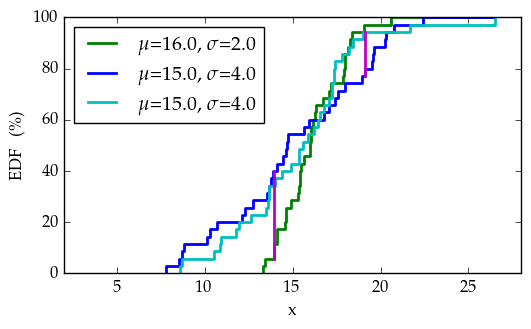
\includegraphics[width=0.9\textwidth]{kuvat/kstest.png}
   \caption{KS test parameter values (magenta vertical lines) shown graphically for three samples from figure \ref{fig:edf}.}
   \label{fig:ks} 
\end{figure}

As an example, let's consider two pairs of samples from figure \ref{fig:edf}: green and blue (two samples drawn from different normal distributions) and blue and cyan (two samples drawn from same normal distribution). We can formulate the test and null hypotheses for both pairs as $H_0$=''the two samples are drawn from the same distribution'' and $H_1$=''the two samples are not drawn from the same distribution'' and choose a significance level of for example $\alpha=0.05$ or $\alpha=0.01$.

\reversemarginpar
\marginnote{\footnotesize{mistä p-value saadaan, kerro taas aiemmin (tai täällä)}}
The test statistic is then calculated and for these samples we get $D=0.51$ for the green-blue pair and $D=0.20$ for the blue-cyan pair. Test statistics are illustrated in figure \ref{fig:ks} where the test statistics $D$ are shown as vertical magenta lines. These values of $D$ correspond to p-values $9.9\times 10^{-5}$ and $0.44$ respectively, which means that the null hypothesis ''green and blue samples are drawn from the same distribution'' is rejected at both 0.05 and 0.01 significance levels but the null hypothesis ''blue and cyan samples are drawn from the same distribution'' cannot be rejected.

\begin{figure}
   \centering
   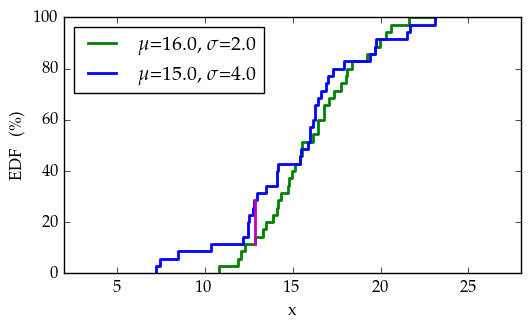
\includegraphics[width=0.9\textwidth]{kuvat/kstest-error.png}
   \caption{KS test ran on another pair of samples drawn from blue and green distributions in figure \ref{fig:cdf}.}
   \label{fig:ks-error} 
\end{figure}

In this case the KS test produced result that matches the actual distributions from which the samples were drawn. Using a different random realization might have resulted in a different conclusion, for example one shown in figure \ref{fig:ks-error} results in $D=0.17$ that corresponds to a p-value of $0.64$ i.e. null hypothesis could not have been rejected using the $\alpha$ specified earlier. In a similar manner there can be cases where two samples from one distribution are erroneously determined not to come from the same distribution if the samples differ from each other enough due to random effects.

The latter example case also illustrates one major shortcoming of the KS test: it is not very sensitive to small-scale differences near the tails of the distribution. For example in figure \ref{fig:ks-error} the blue sample goes much further left, but because EDF is always zero at the lowest allowed value and one at the highest one the vertical distances near the tails are small and the test is most sensitive to differences near the median value of the distribution. On the other hand, the test performs quite well when the samples differ globally or have different means. \citep{feigelson2012modern}

\reversemarginpar
\marginnote{\footnotesize{"explain better"}}[1.8cm]
The KS test is also subject to some limitations and it is important to be aware of them in order to avoid misusing it. First of all, the KS test is not distribution free if the model parameters, e.g. mean and standard deviation for normal distribution, are estimated from the dataset that is tested. Thus the tabulated critical values can be used only if model parameters are determined from some other source such as a simulation, theoretical model or another dataset. \citep{feigelson2012modern}

Another severe limitation of KS test is that it is only applicable to one-dimensional data. If the dataset has two or more dimensions, there is no unique way of ordering the points to plot EDF and therefore if KS test is used, it is no longer distribution free. Some variants that can handle two or more dimensions have been invented, such as ones by \citet{peacock1983twodimensional} and \citet{fasano1987multidimensional}, but the authors do not provide formal proof of validity of these tests. Despite this, the authors claim that Monte Carlo simulations suggest that the methods work adequately well for most applications. \citep{press2007numerical}

% mutlidimensionaaleista http://articles.adsabs.harvard.edu/cgi-bin/nph-iarticle_query?1987MNRAS.225..155F&defaultprint=YES&filetype=.pdf ja http://articles.adsabs.harvard.edu/cgi-bin/nph-iarticle_query?1983MNRAS.202..615P&defaultprint=YES&filetype=.pdf


\subsection{Other tests based on EDFs}
\reversemarginpar
\marginnote{\footnotesize{ehkä vähän lyhyenpuoleisia kappaleita}}
Unsatisfactory sensitivity of the KS test motivates the use of other more complex tests. Such tests are for example the Cram\'er-von Mises test (CvM) and Anderson-Darling (AD) test, both of which have their strengths. Similar to KS test, both of these can be used as one-sample or two-sample variants.  \citep{bohm2010introduction, feigelson2012modern}

First of these tests integrates over the squared difference between the EDF of the sample and CDF from the model or two EDFs in case of two-sample test. The test statistic $W^2$ for one-sample case can be expressed formally as
\begin{equation}
	W^2 = \int_{-\infty}^{\infty}[\hat F_1(x) - F_0(x)]^2\ dF_0(x)
\end{equation}
For two-sample version, the theoretical CDF $F_0$ has to be replaced with another empirical distribution function $\hat F_2$. \citep{bohm2010introduction, feigelson2012modern}

Due to integration, the CvM test is able to differentiate distributions based on both local and global differences, which causes it to often perform better than the KS test. Similar to the KS test, the CvM test also suffers from EDFs or an EDF and a CDF being equal at the ends of the data range, which again makes the test less sensitive to differences near the tails of the distribution. \citep{feigelson2012modern}

In order to achieve constant sensitivity over the entire range of values, the statistic has to be weighted according to the proximity of the ends of the distribution. The AD test does this with its test statistic defined as
\begin{equation}
	A^2 = N \int_{-\infty}^{\infty} \frac{[\hat F_1(x) - F_0(x)]^2}{F_0(x)[1-F_0(x)]}\ dF_0(x)
\end{equation}
where $N$ is the number of data points in sample. This weighing makes the test more powerful than the KS and CvM tests in many cases. \citep{bohm2010introduction, feigelson2012modern}

\reversemarginpar
\marginnote{\footnotesize{hnnngh}}
Also other more specific tests exist, such as the Kuiper test which is well suited for cyclic measurements. The test should always be chosen to match the dataset such that it best differentiates between the null and research hypotheses. \citep{bohm2010introduction, feigelson2012modern}

\section{Cluster Analysis}
DBSCAN

\chapter{Findings from DMO Halo Catalogue Analysis}
\section{Selection of Local Group analogues}
criteria, how many found, what are like (some plots maybe? distributions of masses, separations, velocity components, number of subhaloes within some radius or correlations between two of those?). Some of this might be part of previous chapter too (relevant to resimulation)?

\reversemarginpar
\marginnote{\footnotesize{TODO: selitykset sille, miten osa on keskittynyt tiettyihin arvoihin sallitulla välillä ja osa jakautunut tasaisemmin. Mieti, pitäisikö kolme viimeistä esittää esim scatterplottina combined mass vs mass in more massive}}
Figure \ref{fig:LGproperties} shows how different features of the found LG analogues are distributed. TODO: selitykset sille, miten osa on keskittynyt tiettyihin arvoihin sallitulla välillä ja osa jakautunut tasaisemmin. 

\begin{figure}
    \centering
    %\def\svgwidth{\columnwidth}
    \input{kuvat/tex/LGproperties.pdf_tex}
    \caption{Distributions of LG analogue properties. TODO: selitä, mieti miten y-akselin label, binien rajat pitäisi pakottaa suurimpaan ja pienimpään sallittuun arvoon}\label{fig:LGproperties}
\end{figure}


\section{Hubble Flow Measurements}
HF, local $H_0$, $H_0$ within shells, zero-point, are previous consistent with what went into the simulation

Figure \ref{fig:hubblediagrams}: two different simulations, MW-centered, huom obs nb how different they are: scatter, number of haloes, changes in scatter (bound structures)

\begin{figure}
    \centering
    %\def\svgwidth{\columnwidth}
    \input{kuvat/tex/hubblediagrams.pdf_tex}
    \caption{Hubble Flows around Milky Way in two simulations.}\label{fig:hubblediagrams}
\end{figure}

Figure \ref{fig:hubblefit} shows haloes included and excluded in fitting, how is the process done

\begin{figure}
    \centering
    %\def\svgwidth{\columnwidth}
    \input{kuvat/tex/hubblefit.pdf_tex}
    \caption{HF slope: 86.9929348817}\label{fig:hubblefit}
\end{figure}

Figure \ref{fig:shelledH0} shows H0 at different radii. First bump is clear, latter ones not, H0>67.7 km/s, why. First ones have ~350 samples, last ones only seven, remember to explain standard error. Figure \ref{fig:zeros} has bigger bins and shows zero points. Think whether both should use samy plot type and which is better (line vs boxplot). If boxplot stays, change colours to all-black? At least explain what is what in plot.

\begin{figure}
    \centering
    %\def\svgwidth{\columnwidth}
    \input{kuvat/tex/shelledH0.pdf_tex}
    \caption{Mean H0 in different 2 Mpc bins, grey curves show standard error.}\label{fig:shelledH0}
\end{figure}

\begin{figure}
    \centering
    %\def\svgwidth{\columnwidth}
    \input{kuvat/tex/zeros.pdf_tex}
    \caption{HF zero point in different 4 Mpc bins. specify one outlier outside the plot}\label{fig:zeros}
\end{figure}


X\section{Anisotropy of Hubble flow}
isotropy + randomness or anisotropy? esittele konsepti. plots: see notebook last pages

\reversemarginpar
\marginnote{\footnotesize{Simulaatio 97, esittele jo tässä näkyvät klöntit joissa paljon samaa väriä, näytä myös klusterointi ja vertaa löytöjä siihen}}
Figure \ref{fig:mollweide-anisotropy} shows distribution of haloes around Milky Way analogue from one simulation with haloes closer than 1.5 Mpc away from center excluded to avoid cluttering the view with Andromeda counterpart and its satellites.

\begin{figure}
    \centering
    %\def\svgwidth{\columnwidth}
    \input{kuvat/tex/mollweide-anisotropy.pdf_tex}
    \caption{Projections of haloes around the less massive LG primary with distances ranging from 1.5 Mpc to 5.0 Mpc.}\label{fig:mollweide-anisotropy}
\end{figure}

\subsection{Clustering}
Used DBSCAN introduced in [earlier chapter], angular distances of projections on sky as seen from MW.

Figure \ref{fig:clusteringparameters} shows the effect of varying minsamples and $\varepsilon$ on number of clusters found in each simulation (1.5 Mpc < r < 5.0 Mpc again). Regions where there are ridiculously many clusters and ones where there are one or zero, relevant region in between, some areas have similar number of clusters but do the clusters look the same, see plots that don't exist yet

\begin{figure}
    \centering
    \input{kuvat/tex/clusteringParameters.pdf_tex}
    \caption{Mean number of clusters found for all simulations in dataset with different DBSCAN parameters. In all simulations $\varepsilon$ is scaled using the mean distance between closest neighbours.}\label{fig:clusteringparameters}
\end{figure}

\reversemarginpar
\marginnote{\footnotesize{TODO: mieti laitatko samaan figureen, vertaile kuitenkin, selitä vasemmanpuolimmainen pikselisarake}}
Figure \ref{fig:clusterdiameter} shows the change in mean diameter (supremum of angular distance between haloes) in cluster when $\varepsilon$ and minsamples are varied. White areas where no clusters are found in any simulation.

\begin{figure}
    \centering
    \input{kuvat/tex/clusterDiameter.pdf_tex}
    \caption{Mean diameter of clusters found for all simulations in dataset with different DBSCAN parameters. In all simulations $\varepsilon$ is scaled using the mean distance between closest neighbours.}\label{fig:clusterdiameter}
\end{figure}

\reversemarginpar
\marginnote{\footnotesize{Ehkä vähän vähemmän tilaa plottien välissä vaakasuunnassa? Keltaiset vähän turhan samanlaisia.}}
Figures \ref{fig:clusteringExamples} and \ref{fig:clusteringvariations} show how the clustering results vary when clustering parameters are varied.

\begin{figure}
    \centering
    \input{kuvat/tex/clusteringExamples.pdf_tex}
    \caption{Results of DBSCAN clustering on same simulation output with different clustering parameters. TODO: mieti, kuuluuko tämäntyyppinen DBSCANin yleisiä ominaisuuksia esittelevä kuva enemmänkin teoriaosaan. Toisaalta selvästi dataspesifejä juttuja.}\label{fig:clusteringExamples}
\end{figure}

\begin{figure}
    \centering
    \input{kuvat/tex/smallClusteringVariations.pdf_tex}
    \caption{The effect of slightly variying the clustering parameters around the values $\varepsilon$=1.8 and minsamples=10 used when analyzing clustered data.}\label{fig:clusteringvariations}
\end{figure}

\reversemarginpar
\marginnote{\footnotesize{Massakynnys? Kaksi eri kynnystä? Liian kapea ja epätasapainoinen, laita päällekkäin?}}
Figure \ref{fig:clusteredHFparameters} shows how derived values of slope and zero-point for the Hubble flow change when the Hubble flow fitting is carried out on partial data chosen based on the cluster membership of the haloes.

\begin{figure}
    \centering
    \input{kuvat/tex/clusteredHFparameters.pdf_tex}
    \caption{Hubble constant and distance to the point at which velocity due to the fitted Hubble flow is zero calculated from different samples. HUOM OBS NB erittele plotin ulkopuolelle jääneet kaukaiset outlierit}\label{fig:clusteredHFparameters}
\end{figure}

\section{Statistical Estimate of the Local Group Mass}
Analysis similar to Fattahi et al 2016 paper


%\chapter{SIBELIUS project}
% Simulations Beyond the Local Universe
%
%\section{Hubble Flow Fitting}
%
% %if results
%\chapter{Conclusions}

\chapter{Conclusions}





% STEP 5:
% Uncomment the following lines and set your .bib file and desired bibliography style
% to make a bibliography with BibTeX.
% Alternatively you can use the thebibliography environment if you want to add all
% references by hand.

\clearpage
\addcontentsline{toc}{chapter}{Bibliography} % This lines adds the bibliography to the ToC
\bibliographystyle{plainnat}
\bibliography{lahteet}


\end{document}

